\section{Ortopædkirurgisk afdeling på Aalborg Universitetshospital}
Ortopædkirurgisk afdeling på Aalborg Universitetshospital (OA) behandler primært skader på bevægelsesapparatet, herunder knogler, muskler, sener eller led. Afdelingen er delt op i 10 fagområder: Børneortopædkirurgi, knogle- og rekonstruktion, fod- og ankelkirurgi, knæ- og hoftekirurgi, håndkirurgi, ryg- og bækkenkirurgi, knæ- og idrætsskader, tumor- og sarkomkirurgi, amputationer og sår samt traumatologi. Afdelingen er opdelt i fem afsnit herunder Sengeafsnit O1, O2, operationsafsnit, Sammedagskirurgisk afsnit O6 samt ambulatorium. 
Sengeafsnit O1, der bl.a. behandler brud og skader på hånden, lårbenshalsen samt sportskader i knæet. De behandler ligeledes forbrændinger og ætsninger på dette sengeafsnit. Sengeafsnit O2 varetager børneoperationer, ryglidelser, fod- og ankelskader samt bækkenbrud og patienter med mange brud. Operationsafsnittet udfører de længerevarende operationer samt de operationerne, der kræver speciallægeviden. Sammedagskirurgisk afsnit O6 foretager de mindre operative indgreb. Det sidste afsnit, ambulatorium, kontrollerer patienter, der har behov for kontrol før eller efter en operation.\cite{Aalborg2016}

\subsection{Personalets arbejdsgang}
På OA arbejder personalet i gennemsnit 37 timer om ugen\cite{Danske2015} over en periode på 8 uger. Vagterne består både af dag- og nattevagter. Over en arbejdsdag er der indlagt tre vagtskifte, hvor det nye vagthold har et kvarter til at sætte sig ind i, hvilke opgaver samt patienter de skal varetage. Der er indlagt betalte pauser i personalets arbejdedag, hvilket betyder, at personalet skal være til rådighed under pausen. Personalet arbejder ofte i par, hvor de sammen varetager 2-8 patienter om dagen, mens de ofte varetager flere patienter på aftenvagter.\ref{bilagA}

\subsection{Patienter}
OA modtager både elektive samt akutte patienter. Elektive patienter omfatter både indlagte og ambulante patienter. Ved pludselig forværret tilstand kan elektive patienter skifte status fra elektiv til akut. Akutte patienter defineres som personer, der er henvist til hospitalet efter en akut opstået tilstand.\cite{RegionNord2016} En fordeling af de elektive og akutte patienter fremgår af \figref{elektivvsakut}.

\begin{figure}[H]
	\flushleft 
	\centering
	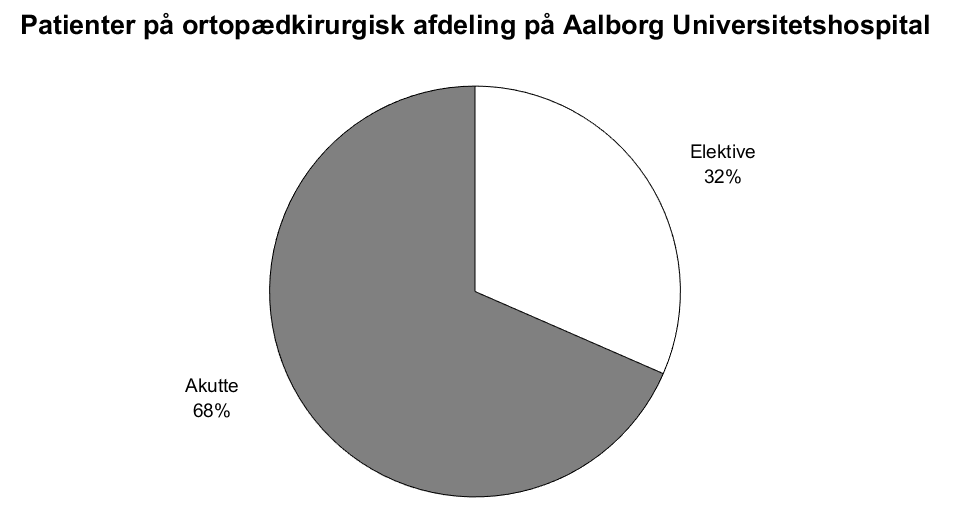
\includegraphics[scale=0.55]{figures/elektivvsakut.png}
	\flushleft
	\caption{\textit{Fordeling af elektive og akutte patienter på OA målt over en tre måneders periode fra juli til og med oktober år 2014.}}
	\label{elektivvsakut}
	\end{figure}

\noindent
Af \figref{elektivvsakut} illustreres det, at fordelingen mellem elektive og akutte patienter ikke er ligeligt fordelt på OA. Der ses over en tre måneders periode i år 2014, at de elektive patienter udgør $32~\%$ og de akutte udgør $68~\%$ af de samtlige patienter. \\

\subsection{Planlægning af patienter} \label{book}
På OA foregår planlægning af elektive patienter med forbehold for akutte patienter, da akutte patienter ikke kan planlægges. Dette betyder, at antallet af sengepladser ikke udnyttes fuldt ud. Operationstiden planlægges ofte ud fra patienternes eget ønske. Det kan være et ønske om en bestemt kirurg, tidsperiode eller blot den første ledige tid.\ref{bilagA} Indlæggelses- og udskrivelsestidspunktet for akutte og elektive i perioden fra juli til og med oktober år 2014 fremgår af \figref{indlaegudskriv}. 

\begin{figure}[H]
	%\flushleft 
	\centering
	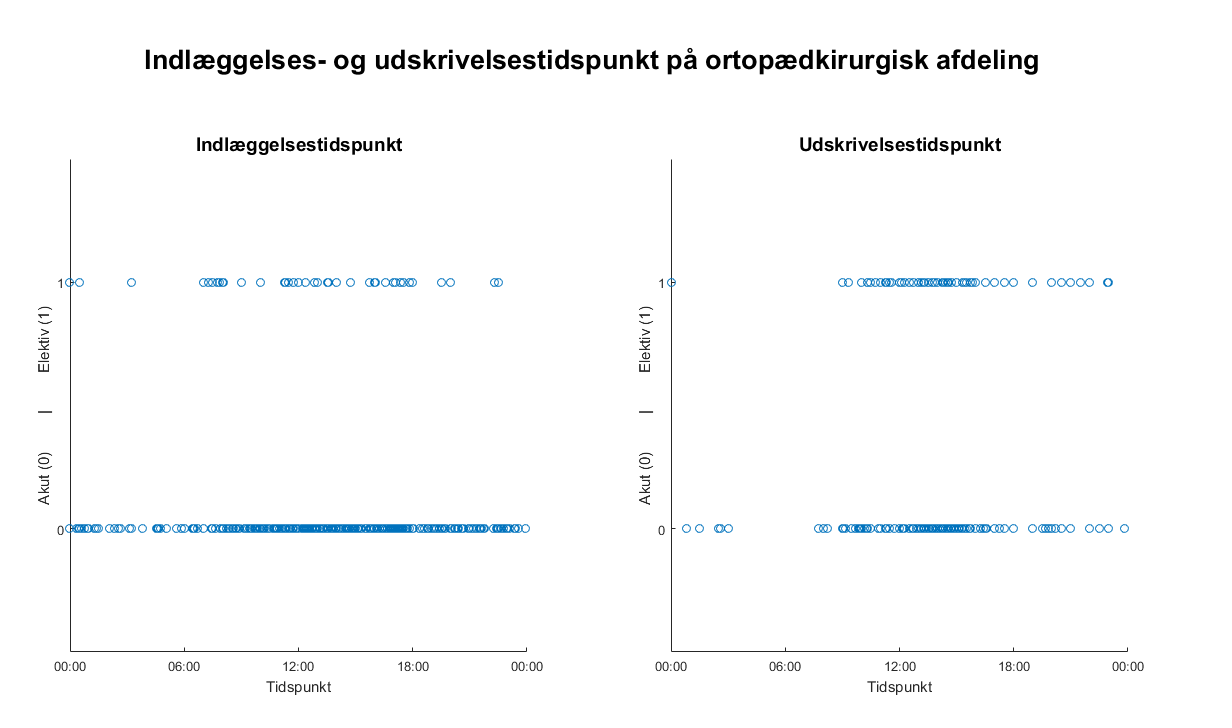
\includegraphics[scale=0.5]{figures/indlaegudskriv.png}
	%\flushleft
	\caption{\textit{Indlæggelse- og udskrivelsestidspunkt for akutte og elektive patienter over en periode fra juli til og med oktober år 2014.}}
	\label{indlaegudskriv}
	\end{figure}
	
\noindent
På \figref{indlaegudskriv} fremgår indlæggelses- og udskrivelsestidspunkter for akutte og elektive patienter. Indlæggelsestidspunktet for elektive ses typisk mellem kl. 7 og 18, hvorimod de akutte indlæggelses i løbet af hele døgnet. Udskrivelsestidspunktet for elektive ses typisk melem kl. 9 og 18, mens akutte typisk udskrives mellem kl. 8 og 18. 

